%==================================================================
%==================================================================
\section{Motif distribution}
\frame{\frametitle{Outline} \tableofcontents[currentsection]}
%==================================================================
\frame{\frametitle{Counting motifs}

  \hspace{-.05\textwidth}
  \begin{tabular}{ll}
    \begin{tabular}{p{.4\textwidth}}
      \paragraph{Number of 'positions'.}
      \begin{itemize}
       \item Choose $p$ nodes among $m$
       \item Choose $q$ nodes among $n$
       \item Try all {\sl automorphisms} 
      \end{itemize}
      $$
      c_s := 
      \left(\begin{array}{c}m \\ p\end{array}\right)
      \times \left(\begin{array}{c}n \\ q\end{array}\right)
      \times r_s
      $$ 
      ~ \\ ~ \\
    \end{tabular}
    & \pause
    \begin{tabular}{p{.5\textwidth}}
      \paragraph{Automorphisms=} non-redundant permutations \\
      \includegraphics[width=.1\textwidth]{\fignet/FigMotifsBEDD-motif9-automorphism1}
      \includegraphics[width=.1\textwidth]{\fignet/FigMotifsBEDD-motif9-automorphism2}
      \includegraphics[width=.1\textwidth]{\fignet/FigMotifsBEDD-motif9-automorphism3} \\
      \includegraphics[width=.1\textwidth]{\fignet/FigMotifsBEDD-motif9-automorphism4}
      \includegraphics[width=.1\textwidth]{\fignet/FigMotifsBEDD-motif9-automorphism5}
      \includegraphics[width=.1\textwidth]{\fignet/FigMotifsBEDD-motif9-automorphism6} 
    \end{tabular} 
  \end{tabular}
  
  \bigskip \bigskip \pause
  \paragraph{Motif count.} Try all positions $\alpha = 1, \dots c_s$, define 
  $$
  Y_{s\alpha} = 1 \text{ if match,} \qquad 0 \text{ otherwise},
  $$
  then count the number of matches:
  $$
  N_s = \sum_\alpha Y_{s\alpha}
  $$
  \ra \emphase{Motif frequency}: $F_s := N_s / c_s$
  
}

% %==================================================================
% \frame{\frametitle{Motif probability}
% 
%   \paragraph{Occurrence probability $\overline{\phi}_s = \Pbb\{Y_{s\alpha} = 1\}$.} Under the B-EDD model \refer{OLR22}:
%   \begin{align*}
%     \overline{\phi}_s 
%     & :=
%     \Pbb_{\BEDD}\left(
%     \includegraphics[width=.06\textwidth, trim=100 200 100 0]{\fignet/FigMotifsBEDD-motif9} 
%     \right)
%     \; = \; 
%     \frac{
%     \onslide+<2->{
%       \overset{\text{top stars}}{\overbrace{
%       \Pbb\left(\includegraphics[width=.05\textwidth, trim=100 200 100 0]{\fignet/FigMotifsBEDD-motif9-top1}\right) % \times 
%       \Pbb\left(\includegraphics[width=.05\textwidth, trim=100 200 100 0]{\fignet/FigMotifsBEDD-motif9-top1}\right) % \times 
%       \Pbb\left(\includegraphics[width=.05\textwidth, trim=100 200 100 0]{\fignet/FigMotifsBEDD-motif9-top2}\right)   }}
%     }
%     \onslide+<3->{
%       \times
%       \overset{\text{bottom stars}}{\overbrace{
%       \Pbb\left(\includegraphics[width=.05\textwidth, trim=100 200 100 0]{\fignet/FigMotifsBEDD-motif9-bottom1}\right) % \times
%       \Pbb\left(\includegraphics[width=.05\textwidth, trim=100 200 100 0]{\fignet/FigMotifsBEDD-motif9-bottom3}\right)
%       }}
%     }
%     }{
%     \onslide+<4->{
%       \underset{\text{edges}}{\underbrace{
%       \left(\Pbb\left(\includegraphics[width=.05\textwidth, trim=100 200 100 0]{\fignet/FigMotifsBEDD-motif9-top1}\right)\right)^4
%       }}
%     }
%     } 
%     \\
%     \onslide+<5->{
%     & =
%     \frac{\left(\phi_1^2 \phi_2\right) \left(\phi_1 \phi_4\right)}{\left(\phi_1\right)^4}
%     \qquad =
%     \frac{\phi_2 \phi_4}{\phi_1}
%     }
%   \end{align*}
% 
%   \onslide+<6->{\bigskip \bigskip 
%   \paragraph{Estimated probability.} 
%   $$
%   \overline{\phi}_s := \frac{\phi_2 \phi_4}{\phi_1}
%   \qquad \rightarrow \qquad 
%   \overline{F}_s := \frac{F_2 F_4}{F_1}
%   $$
%   where $F_1$, $F_2$, $F_4 =$ observed frequencies of  edges, top stars and bottom stars.
%   }
% }

%==================================================================
\frame{\frametitle{Motif probability}

  \paragraph{Occurrence probability $\overline{\phi}_s = \Pbb\{Y_{s\alpha} = 1\}$.} Under the B-EDD model \refer{OLR22}:
  \begin{align*}
    \left(\includegraphics[width=.06\textwidth, trim=100 200 100 0]{\fignet/FigMotifsBEDD-motif9}\right) 
    & = \; 
    \frac{
    \onslide+<2->{
      \overset{\text{top stars}}{\overbrace{
      \left(\includegraphics[width=.05\textwidth, trim=100 200 100 0]{\fignet/FigMotifsBEDD-motif9-top1}\right) % \times 
      \left(\includegraphics[width=.05\textwidth, trim=100 200 100 0]{\fignet/FigMotifsBEDD-motif9-top1}\right) % \times 
      \left(\includegraphics[width=.05\textwidth, trim=100 200 100 0]{\fignet/FigMotifsBEDD-motif9-top2}\right)   }}
    }
    \onslide+<3->{
      \quad
      \overset{\text{bottom stars}}{\overbrace{
      \left(\includegraphics[width=.05\textwidth, trim=100 200 100 0]{\fignet/FigMotifsBEDD-motif9-bottom1}\right) % \times
      \left(\includegraphics[width=.05\textwidth, trim=100 200 100 0]{\fignet/FigMotifsBEDD-motif9-bottom3}\right)
      }}
    }
    }{
    \onslide+<4->{
      \underset{\text{edges}}{\underbrace{
      \left(\includegraphics[width=.05\textwidth, trim=100 200 100 0]{\fignet/FigMotifsBEDD-motif9-top1}\right)^4
      }}
    }
    } 
    \\
    \onslide+<5->{
    \overline{\phi}_s 
    =
    \Pbb_{\BEDD}\left(
    \includegraphics[width=.06\textwidth, trim=100 200 100 0]{\fignet/FigMotifsBEDD-motif9} 
    \right)
    & = \;
    \frac{\left(\phi_1^2 \phi_2\right) \left(\phi_1 \phi_4\right)}{\left(\phi_1\right)^4}
    \qquad =
    \frac{\phi_2 \phi_4}{\phi_1}
    }
  \end{align*}

  \onslide+<6->{\bigskip \bigskip 
  \paragraph{Estimated probability $\overline{F}_s$.} 
  $$
  \overline{\phi}_s := \frac{\phi_2 \phi_4}{\phi_1}
  \qquad \rightarrow \qquad 
  \overline{F}_s := \frac{F_2 F_4}{F_1}
  $$
  where $F_1$, $F_2$, $F_4 =$ observed frequencies of  edges, top stars and bottom stars.
  }
}

%==================================================================
\frame{\frametitle{Moments of the count} \label{sec:motifMoments}

  \begin{itemize}
  \setlength{\itemsep}{1.5\baselineskip}
  \item \emphase{Number of positions:} $c_s$ 
  \item \emphase{Mean:} $\Esp_{\BEDD}(N_s) = c_s \times \overline{\phi}_s$ 
  \item \pause \emphase{Variance:} Same game, requires to evaluate $\displaystyle{\Esp_{\BEDD}(N_s ^2) = \Esp_{\BEDD}\left(\sum_\alpha Y_{s\alpha} \right)^2}$ \\
  \ra Need to account for overlap between positions ({\sl super-motifs}: \refer{PDK08} \goto{back:superMotifs}) 
  $$
  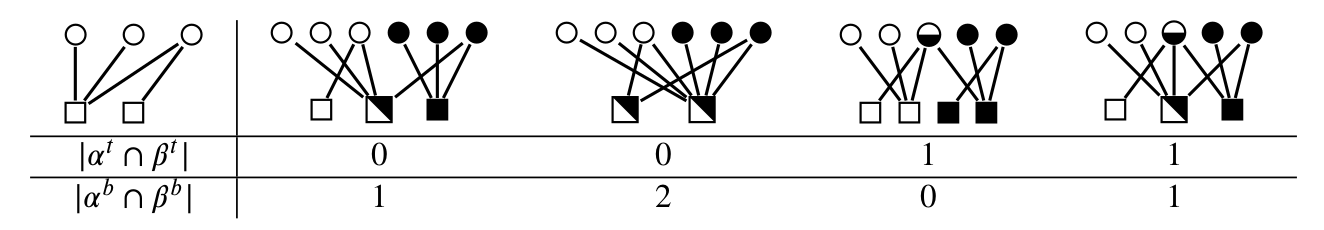
\includegraphics[width=.8\textwidth, trim=0 25 0 0, clip=]{\fignet/OLR22-EJS-Fig2}
  $$ 
  \ra Compute the respective expected count in the way as for regular motifs \\ ~
  \item \pause \emphase{Covariance:} Same game to compute $\Cov(N_s, N_{s'})$
  \item \pause \emphase{Asymptotic normality:} \goto{back:motifDistrib} \goto{back:asymNormality}
  $
  (F_s - \overline{F}_s) \left/ \sqrt{\widehat{\Var}(F_s)} \right. \quad \overset{m, n \rightarrow \infty}{\longrightarrow} \quad \Ncal(0, 1)
  $ 
  \end{itemize}

}

% %==================================================================
% \frame{\frametitle{Distribution of the count}
% 
%   \paragraph{Asymptotic normality for non-star motifs.} Under \BEDD (and sparsity conditions):
%   $$
%   (F_s - \overline{F}_s) \left/ \sqrt{\widehat{\Var}(F_s)} \right. \quad \overset{m, n \rightarrow \infty}{\longrightarrow} \quad \Ncal(0, 1)
%   $$
%   Proof \refer{OLR22}: 
%   \begin{equation*}
%     \text{decompose} \qquad
%    F_s - \overline{F}_s 
%    = \underset{\text{random fluctuations}}{\underbrace{(F_s - \phi_s)}} 
%    + \underset{\text{null under \BEDD}}{\underbrace{(\phi_s - \overline{\phi}_s)}}  
%    + \underset{\text{estimation error } \rightarrow 0}{\underbrace{(\overline{\phi}_s - \overline{F}_s)}}, 
%   \end{equation*}
%   + construct a counting martingale for $F_s - \phi_s$  \refer{GaL17b}.
%   
%   \bigskip \bigskip \pause
%   \paragraph{Consequence.} We know 
%   \begin{itemize}
%     \item the expected behavior (mean, variance, distribution) of any motif count 
%     \item under the BEDD model (= 'null model').
%   \end{itemize}
% }
% 
